\documentclass[a4paper,12pt]{article}
\usepackage[portuguese]{babel}
\usepackage{amsmath,amsthm,amssymb,mathtools,tikz,graphicx,pgfplots,verbatim,fancyhdr}
\pagestyle{fancy}%Style of page
\setlength{\headsep}{0.5in}

\lhead{%Header left
	Universidade Federal da Para\'iba \\
	Discente: Jefferson Bezerra dos Santos\\
	Docente: Jos\'e Miguel Aroztegui Massera 
}

\title{ Lista de EDO aplicada}
\date{\vspace{-5ex}}

\begin{document}
\maketitle\thispagestyle{fancy}
\textbf{1. Quest\~ao:}\\

De fato, o m\'etodo de Runge-Kutta \'e definido como,\\
\begin{align*}
	y_{n+1} - y_{n} &= h\phi(x_{n},y_{n},h)\\
	\phi(x,y,h) &= {c_1}{k_1} + {c_2}{k_2} + \dots + {c_R}{k_R}\\
	k_1 &= f(x,y)\\ 
	k_2 &= f(x + a_2 h,y + hb_{21}{k_1})\\ 
	& \hspace{5pt}\vdots  \\
	k_R &= f(x + a_R h,y + hb_{R1}{k_1} + hb_{R2}{k_2} + \dots + hb_{RR-1}{k_{R-1}})\\ 
\end{align*}
onde:\\
\begin{itemize}
	\item $\phi :\mathbb{R}^{3} \rightarrow \mathbb{R}$;
	\item $a,c$ s\~ao vetores do $\mathbb{R}^{R}$; 
	\item $B$ \'e uma matriz de diagonal inferior em $\mathbb{R}^{\mathrm{RxR}}$.
\end{itemize}
para que o m\'etodo seja consistente deve-se ter o \'indice de erro $q$ maior ou igual a 1. Pela defini\c c\~ao do
m\'etod de Runge-Kutta segue que
\begin{align*}
	C_0 = {\alpha}_0 + {\alpha}_1 = -1 + 1 = 0
\end{align*}
pela defini\c c\~ao de consist\^encia segue que,
\begin{align*}
	C_1 = 0 &\Rightarrow {\alpha}_{1} - ({\beta}_{0} + {\beta}_{1} + \dots + {\beta}_{n} ) = 0 \\
	&\Rightarrow 1 -(c_1 + c_2 + \dots + c_R) = 0  \\
	&\Rightarrow 1 -(c_1 + c_2 + \dots + c_R) = 0  \\
	&\Rightarrow c_1 + c_2 + \dots + c_R = 1 
\end{align*}

\textbf{2. Quest\~ao:}\\
O m\'etodo de Runge-kutta de ordem 3 \'e definido como,\\
\begin{align*}
	y_{n+1} - y_{n} &= h\phi(x_{n},y_{n},h)\\
	\phi (x,y,h) &= {c_1}{k_1} + {c_2}{k_2} + {c_3}{k_3}\\
	k_1 &= f(x,y)\\ 
	k_2 &= f(x + a_2 h,y + hb_{21}{k_1})\\ 
	k_3 &= f(x + a_3 h,y + hb_{31}{k_1} + hb_{32}{k_2}).\\ 
\end{align*}
onde:\\
\begin{itemize}
	\item $\phi :\mathbb{R}^{3} \rightarrow \mathbb{R}$;
	\item $a,c$ s\~ao elementos do $\mathbb{R}^{R}$; 
	\item $b$ \'e uma matriz de diagonal superior em $\mathbb{R}^{\mathrm{RxR}}$.
\end{itemize}
sobre o vetor $a$ \'e imposta a seguinte condi\c c\~ao,
\begin{align*}
	a_1 &= 0\\
	a_2 &= b_{21}\\
	a_3 &= b_{31} + b_{32}\\
\end{align*}
os dados do vetores $a, c$ e da matrix $B$ podem ser organizados da seguinte maneira,
{\arraycolsep=3.4pt\def\arraystretch{1.4}
\[
	\begin{array}{l|ccc} 
		0 &  & & \\
		a_2 & b_{21} & & \\
		a_3 & b_{31} & b_{32}& \\
		\hline
		&c_1 & c_2 & c_3
	\end{array}
\]
}
finalmente o Runge-Kutta de ordem 3 deve satisfazer as seguintes rela\c c\~oes,
\begin{align*}
	c_1 + c_2 + c_3 &= 1 \\
	c_2 a_2 + c_3 a_3 &= \frac{1}{2} \\
	c_2 {a_2}^{2} + c_3 {a_3}^{2}&= \frac{1}{3} \\
	c_3 b_{32} a_2 &= \frac{1}{6}
\end{align*}
\textbf{3. quest\~ao:}\\

{\arraycolsep=3.4pt\def\arraystretch{1.4}
\[
	\begin{array}{l|ccc} 
		0 &  & & \\
		\frac{1}{3} & \frac{1}{3} & & \\
		\frac{2}{3} & 0 & \frac{2}{3}& \\
		\hline
		&\frac{1}{4} & 0 & \frac{1}{4}
	\end{array}
\]
}
verificando as rela\c c\~oes para (Heun),
\begin{align*}
	c_1 + c_2 + c_3 &= \frac{1}{4} + 0 + \frac{3}{4} = 1 \hspace{2pt}(\textrm{v\'alida})\\
	c_2 a_2 + c_3 a_3 &= 0\left (\frac{1}{2} \right) + \frac{3}{4} \left (\frac{2}{3} \right ) = \frac{1}{2} \hspace{2pt}(\textrm{v\'alida})\\
	c_2 {a_2}^{2} + c_3 {a_3}^{2}&= 0 \left ( \frac{1}{3}\right )^{2} +  \frac{3}{4} \left ( \frac{2}{3}\right )^{2} =
	\frac{1}{3}\hspace{2pt}(\textrm{v\'alida})\\ 
	c_3 b_{32} a_2 &=\left (\frac{3}{4}\right )\left (\frac{2}{3}\right )\left (\frac{1}{3}\right ) =
	\frac{1}{6}\hspace{2pt}(\textrm{v\'alida}).
\end{align*}

verificando as rela\c c\~oes para (Nystron),

{\arraycolsep=3.4pt\def\arraystretch{1.4}
\[
	\begin{array}{l|ccc} 
		0 &  & & \\
		\frac{2}{3} & \frac{2}{3} & & \\
		\frac{2}{3} & 0 & \frac{2}{3}& \\
		\hline
		&\frac{1}{4} & \frac{3}{8} & \frac{3}{8}
	\end{array}
\]
}
\begin{align*}
	c_1 + c_2 + c_3 &= \frac{1}{4} + \frac{3}{8} + \frac{3}{8} = \frac{2}{8} + \frac{3}{8} + \frac{3}{8} = 1 \hspace{2pt}(\textrm{v\'alida})\\
	c_2 a_2 + c_3 a_3 &= \frac{3}{8}\left (\frac{2}{3} \right) + \frac{3}{8} \left (\frac{2}{3} \right ) =
	\frac{1}{4} + \frac{1}{4} = \frac{1}{2} \hspace{2pt}(\textrm{v\'alida})\\
	c_2 {a_2}^{2} + c_3 {a_3}^{2}&= \frac{3}{8} \left ( \frac{2}{3}\right )^{2} +  \frac{3}{8} \left ( \frac{2}{3}\right )^{2} =
	\frac{2}{6} = \frac{1}{3}\hspace{2pt}(\textrm{v\'alida})\\ 
	c_3 b_{32} a_2 &=\left (\frac{3}{8}\right )\left (\frac{2}{3}\right )\left (\frac{2}{3}\right ) =
	\frac{1}{2}\left ( \frac{1}{3}\right ) = \frac{1}{6}\hspace{2pt}(\textrm{v\'alida})
\end{align*}
\newpage
\textbf{4. Quest\~ao:}\\
O m\'etodo de Runge-Kutta de 4 ordem \'e definido por,
\begin{align*}
	y_{n+1} - y_{n} &= h\phi(x_{n},y_{n},h)\\
	\phi (x,y,h) &= {c_1}{k_1} + {c_2}{k_2} + {c_3}{k_3} + {c_4}{k_4} \\
	k_1 &= f(x,y)\\ 
	k_2 &= f(x + a_2 h,y + hb_{21}{k_1})\\ 
	k_3 &= f(x + a_3 h,y + hb_{31}{k_1} + hb_{32}{k_2})\\ 
	k_4 &= f(x + a_4 h,y + hb_{41}{k_1} + hb_{42}{k_2}) + hb_{43}{k_3}) .\\ 
\end{align*}
onde:\\
\begin{itemize}
	\item $\phi :\mathbb{R}^{3} \rightarrow \mathbb{R}$;
	\item $a,c$ s\~ao elementos do $\mathbb{R}^{R}$; 
	\item $b$ \'e uma matriz de diagonal superior em $\mathbb{R}^{\mathrm{RxR}}$.
\end{itemize}
sobre o vetor $a$ \'e imposta a seguinte condi\c c\~ao,
\begin{align*}
	a_1 &= 0\\
	a_2 &= b_{21}\\
	a_3 &= b_{31} + b_{32}\\
	a_4 &= b_{41} + b_{42} + b_{43}\\
\end{align*}
os dados do vetores $a, c$ e da matrix $b$ podem ser organizados da seguinte maneira,
{\arraycolsep=3.4pt\def\arraystretch{1.4}
\[
	\begin{array}{l|cccc} 
		0 &  & & \\
		a_2 & b_{21} & & & \\
		a_3 & b_{31} & b_{32}& &\\
		a_4 & b_{41} & b_{42}&b_{43} &\\
		\hline
		&c_1 & c_2 & c_3 & c_4
	\end{array}
\]
}
finalmente o Runge-Kutta de ordem 3 deve satisfazer as seguintes rela\c c\~oes,
\begin{align*}
	c_1 + c_2 + c_3 + c_4 &= 1 \\
	c_2 a_2 + c_3 a_3  + c_4 a_4&= \frac{1}{2} \\
	c_2 {a_2}^{2} + c_3 {a_3}^{2} + c_4 {a_4}^{2}&= \frac{1}{3} \\
	c_3 b_{32} a_2 + c_4 b_{42}a_2  + c_4 b_{43} a_3 &= \frac{1}{6}\\
	c_2 {a_2}^{3} + c_3 {a_3}^{3} + c_4 {a_4}^{3}&= \frac{1}{4} \\
	c_3 a_3 b_{32} a_2 + c_4 a_4 b_{42}a_2  + c_4 a_4 b_{43} a_3 &= \frac{1}{8}\\
	c_4 b_{43} b_{32} a_2 &= \frac{1}{24}
\end{align*}
\textbf{5. Quest\~ao:}\\
Dada a configura\c c\~ao 3 abaixo, vamos verificar as rela\c c\~oes do Runge-Kutta de 4 ordem.
{\arraycolsep=3.4pt\def\arraystretch{1.4}
\[
	\begin{array}{l|cccc} 
		0 &  & & \\
		\frac{1}{2} & \frac{1}{2} & & & \\
		\frac{1}{2} & 0 & \frac{1}{2}& &\\
		1 & 0 & 0 & 1 &\\
		\hline
		&\frac{1}{6} & \frac{1}{3} & \frac{1}{3} & \frac{1}{6}
	\end{array}
\]
}
verificando,
\begin{align*}
	c_1 + c_2 + c_3 + c_4 &= \frac{1}{6} + \frac{1}{3} + \frac{1}{3} + \frac{1}{6}= \frac{2}{6} +
	\frac{4}{6}=  1\hspace{2pt}(\textrm{v\'alida}) \\
	c_2 a_2 + c_3 a_3  + c_4 a_4&= \frac{1}{3}\left (\frac{1}{2} \right ) + \frac{1}{3} \left
	(\frac{1}{2}\right ) +\frac{1}{6} = \frac{2}{6} +\frac{1}{6} =\frac{1}{2} \hspace{2pt}(\textrm{v\'alida})\\
	c_2 {a_2}^{2} + c_3 {a_3}^{2} + c_4 {a_4}^{2}&=  \frac{1}{3}\left (\frac{1}{4}\right ) + \frac{1}{3}\left
	(\frac{1}{4}\right ) + \frac{1}{6} = \frac{1}{6} + \frac{1}{6}= \frac{1}{3} (\textrm{v\'alida})\\
	c_3 b_{32} a_2 + c_4 b_{42}a_2  + c_4 b_{43} a_3 &= \frac{1}{3} \left  (\frac{1}{2}\right ) \left
	(\frac{1}{2}\right ) + \frac{1}{6} (0)\left (\frac{1}{2}\right ) + \frac{1}{6}(1)\left (\frac{1}{2}\right )  =
	\frac{2}{12}=\frac{1}{6}\hspace{2pt}(\textrm{v\'alida})\\
	c_2 {a_2}^{3} + c_3 {a_3}^{3} + c_4 {a_4}^{3}&= \frac{1}{3} \left (\frac{1}{8}\right ) + \frac{1}{3}\left
	( \frac{1}{8}\right )  + \frac{1}{6} =  \frac{3}{12}=\frac{1}{4}(\textrm{v\'alida}) \\
	c_3 a_3 b_{32} a_2 + c_4 a_4 b_{42}a_2  + c_4 a_4 b_{43} a_3 &=  \frac{1}{3}\left (\frac{1}{2}\right)\left
	(\frac{1}{2}\right)\left (\frac{1}{2}\right) + 0  \frac{1}{12} + = \frac{3}{24} = \frac{1}{8}(\textrm{v\'alida})\\
	c_4 b_{43} b_{32} a_2 &=  \frac{1}{6} (1)\left (\frac{1}{2} \right )\left (\frac{1}{2} \right ) = \frac{1}{24}(\textrm{v\'alida})
\end{align*}
Dada a configura\c c\~ao 4 abaixo, vamos verificar as rela\c c\~oes do Runge-Kutta de 4 ordem.

{\arraycolsep=3.4pt\def\arraystretch{1.4}
\[
	\begin{array}{l|cccc} 
		0 &  & & \\
		\frac{1}{3} & \frac{1}{3} & & & \\
		\frac{2}{3} & -\frac{1}{3} & 1& &\\
		1 & 1 & -1 & 1 &\\
		\hline
		&\frac{1}{8} & \frac{3}{8} & \frac{3}{8} & \frac{1}{8}
	\end{array}
\]
}
verificando,
\begin{align*}
	c_1 + c_2 + c_3 + c_4 &=  \frac{1}{8} + \frac{3}{8} + \frac{3}{8} + \frac{1}{8} = 1 (\textrm{v\'alida}) \\
	c_2 a_2 + c_3 a_3  + c_4 a_4&= \frac{3}{8}\left (\frac{1}{3}\right ) + \frac{3}{8}\left (\frac{2}{3} \right )
	 +  \frac{1}{8}= \frac{4}{8} = \frac{1}{2} (\textrm{v\'alida})\\
	 c_2 {a_2}^{2} + c_3 {a_3}^{2} + c_4 {a_4}^{2}&= \frac{3}{8}{\left (\frac{1}{3}\right )}^{2} + \frac{3}{8}{\left
		 (\frac{2}{3} \right )}^{2}
		 +  \frac{1}{8} = \frac{1}{24} + \frac{4}{24} + \frac{3}{24} = \frac{1}{3} (\textrm{v\'alida})\\
		 c_3 b_{32} a_2 + c_4 b_{42}a_2  + c_4 b_{43} a_3 &= \frac{3}{8} (1)\left ( \frac{1}{3}\right ) + \frac{1}{8}
		 (-1)\left ( \frac{1}{3}\right ) + \frac{1}{8} (1)\left ( \frac{2}{3}\right ) = \frac{4}{24}= \frac{1}{6}(\textrm{v\'alida})\\
	c_2 {a_2}^{3} + c_3 {a_3}^{3} + c_4 {a_4}^{3}&=  \frac{3}{8}{\left (\frac{1}{3}\right )}^{3} + \frac{3}{8}{\left
		 (\frac{2}{3} \right )}^{3}
		 = \frac{2}{8}= \frac{1}{4} (\textrm{v\'alida})\\
	c_3 a_3 b_{32} a_2 + c_4 a_4 b_{42}a_2  + c_4 a_4 b_{43} a_3 &= \frac{3}{8}\left (\frac{2}{3}\right ) (1)\left (\frac{1}{3}\right ) 
	+ \frac{1}{8}(1) (-1)\left (\frac{1}{3}\right ) + \frac{1}{8}(1) (1)\left (\frac{2}{3}\right ) = \frac{1}{8}(\textrm{v\'alida})\\
	c_4 b_{43} b_{32} a_2 &= \frac{1}{8} (1) (1)\left ( \frac{1}{3}\right ) = \frac{1}{24}(\textrm{v\'alida})
\end{align*}

\textbf{6. Quest\~ao:}\\

1) A fun\c c\~ao incognita1 \'e o Range-Kutta de ordem R que calcular o vetor coluna para a solu\c c\~ao do sistema de equa\c
c\~oes diferencias. \\

2)
A fun\c c\~ao incognita2 \'e o m\'etodo de Heun um Runge-Kutta de ordem 3 que calcular a matriz solu\c c\~ao do sistema
de equa\c c\~oes, a fun\c c\~ao incognita2 carregar os dados necess\'arios para aplicar a fun\c c\~ao Runge-Kutta de
ordem R, isto \'e os vetores $a,c$ e a matriz $B$. \\

3) Mudaria os vetores a,c e matriz B, isto \'e
{\arraycolsep=3.4pt\def\arraystretch{1.4}
\begin{align*}
	 a = \left [
		 \begin{array}{c}	
			 0 \\
			 \frac{2}{3} \\
			 \frac{2}{3} 
\end{array} \right 
], 
c =\left [
	\begin{array}{ccc} 
		\frac{1}{4} & \frac{3}{8} & \frac{3}{8}
\end{array}
\right ] 
e \hspace{2pt} 
B =\left [
	\begin{array}{cc} 
		 \frac{2}{3} & 0 \\ 
		0 & \frac{2}{3}\\ 
\end{array}
\right 
]
\end{align*}
}

\textbf{7. Quest\~ao:}\\
Para facilitar a transforma\c c\~ao do problema (5) esse ser\'a reescrito da seguinte forma, 
\[\left \{
	\begin{array}{ccc}
	{\theta}^{''}(x)& = & -\frac{g}{d} sen(\theta(x)) \\
	{\theta}^{'}(0) &  = & 0 \\
	{\theta}(0) &= & \frac{\pi}{3} 
\end{array}
\right .
 \]
Para transformar o problema (5) em um sistema de equa\c c\~oes faremos a seguinte substitui\c c\~ao,
\begin{align*}
	y_1 = \theta \hspace{3pt} & \Rightarrow  {y_1}^{'} = y_2\\
	y_2 = {\theta}^{'} & \Rightarrow  {y_2}^{'} = y_3 \\
	y_3 = {\theta}^{''} & 
\end{align*}
O vetor coluna da matriz solu\c c\~ao do sistema de equa\c c\~oes ser\'a dado por, 
\begin{align*}
	P_c  =  \left [ 
		\begin{array}{c}
			y_1 \\	
			{y_2}	
		\end{array}
	\right ] \hspace{3pt} =\left [ 
		\begin{array}{c}
			\theta \\	
			{\theta}^{'} 	
		\end{array}
	\right ]\hspace{3pt}, \textrm{com a condi\c c\~ao inicial} \hspace{3pt}P_1 =\left [
		\begin{array}{c}	
			\theta (0) \\
			{\theta}^{'} (0)
		\end{array} 
	\right ]   
\end{align*}
a fun\c c\~ao $f$ ser\'a definida como,
$f(t,P_c)=  \left [ 
		\begin{array}{c}
			y_2 \\	
			{y_3}	
		\end{array}
	\right ] \hspace{3pt} =\left [\begin{array}{c}
		p_2 \\
		-\frac{g}{d} sin (p_1)
	\end{array}
\right ] $ onde $p_1$ e $p_2$ s\~ao elementos do vetor coluna $P_c$.
Finalmente a matriz solu\c c\~ao do sistema de  equa\c c\~oes ser\'a dada por,
\begin{align*}
	P =\left [
		\begin{array}{cccc}
			{\theta}_1 & {\theta}_2 & \dots & {\theta}_{N+1} \\
			{{\theta}_1}^{'}& {{\theta}_2}^{'} & \dots & {{\theta}_{N+1}}^{'}
		\end{array}
	\right ] 
\end{align*}
onde por defini\c c\~ao $ {\theta}_1 = \theta (0)$ e ${{\theta}_1}^{'} = {\theta}^{'} (0)$.

\textbf{8. Quest\~ao:}\\
Para est\'a quest\~ao utilizei o m\'etodo que estava j\'a definido, ou seja, o Range-Kutta de ordem 3 o m\'etodo de
Heun.
\verbatiminput{RungeKuttaR.m}
\verbatiminput{Heun.m}
\verbatiminput{pendulo.m}
\begin{figure}[!h]
	\centering
	\resizebox{0.5\width}{!}{
	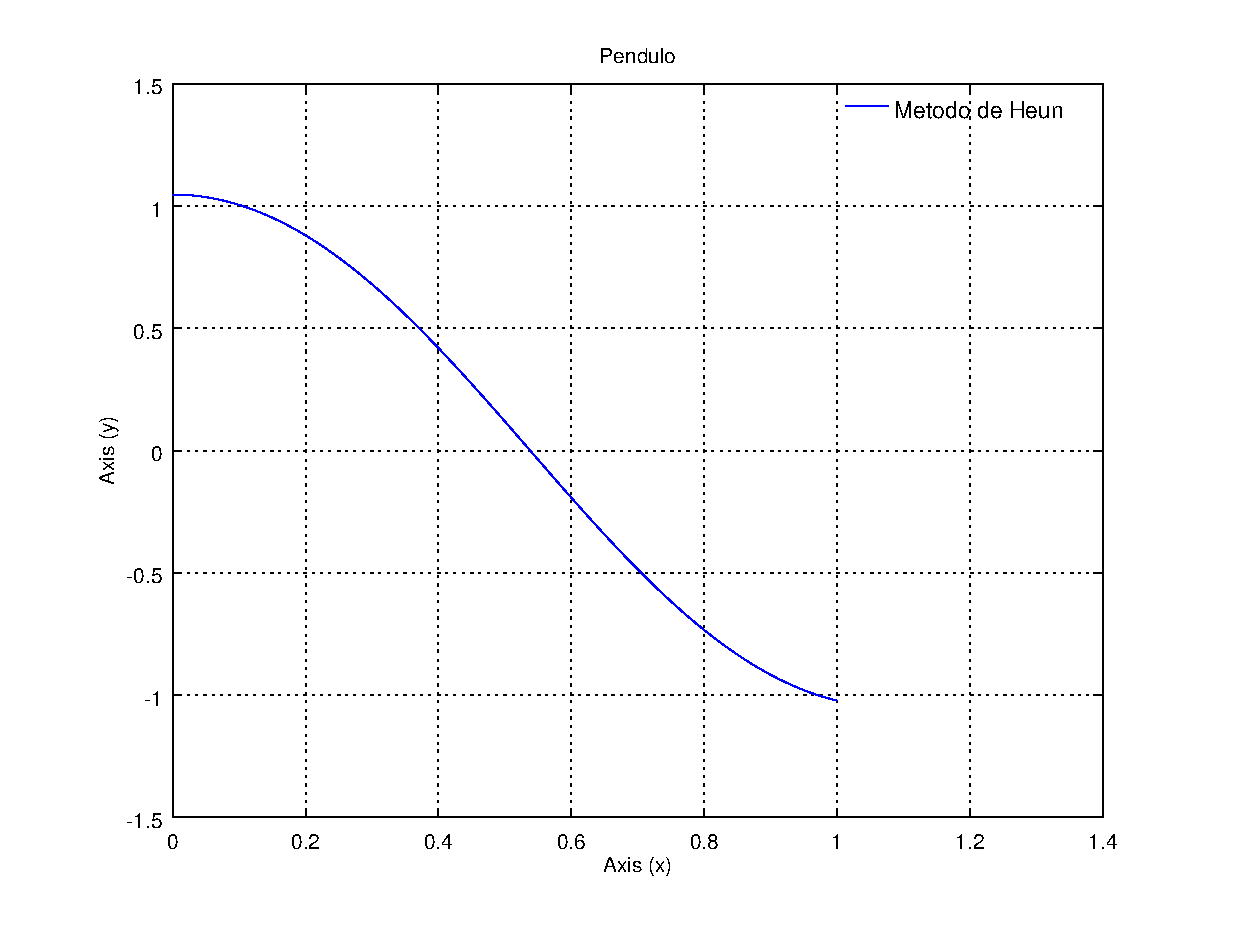
\includegraphics{pen.eps}
	}
\end{figure}

\textbf{9. Quest\~ao:}\\
\verbatiminput{RungeKuttaR.m}
\verbatiminput{Runge4.m}

\textbf{10. Quest\~ao:}\\

\verbatiminput{RungeKuttaR.m}
\verbatiminput{Runge4.m}
\verbatiminput{kepler.m}
O m\'etodo de Kepler com $n = 100$ e $h = 0.1$ para o vetor inicial,
\[\left [ 
	\begin{array}{c}
		1 \\
		0 \\
		1 \\
		1
	\end{array}
\right ] 
\]
\begin{figure}[!h]
	\centering
	\resizebox{0.5\width}{!}{
	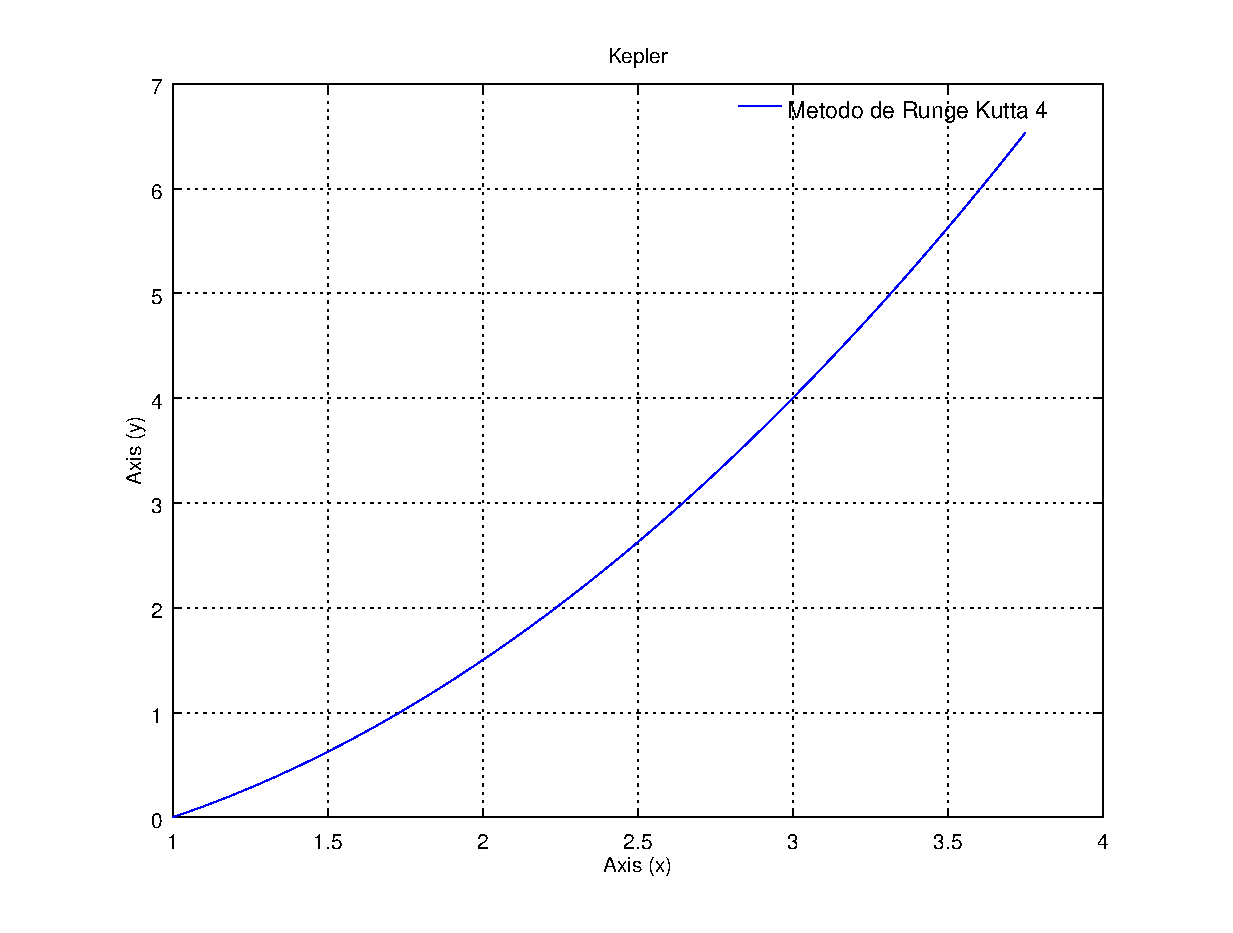
\includegraphics{k1.eps}
	}
\end{figure}
\newpage
O m\'etodo de Kepler com $n = 100$ e $h = 0.1$ para o vetor inicial,
\[\left [ 
	\begin{array}{c}
		1 \\
		0 \\
		0 \\
		1
	\end{array}
\right ] 
\]

\begin{figure}[!h]
	\centering
	\resizebox{0.5\width}{!}{
	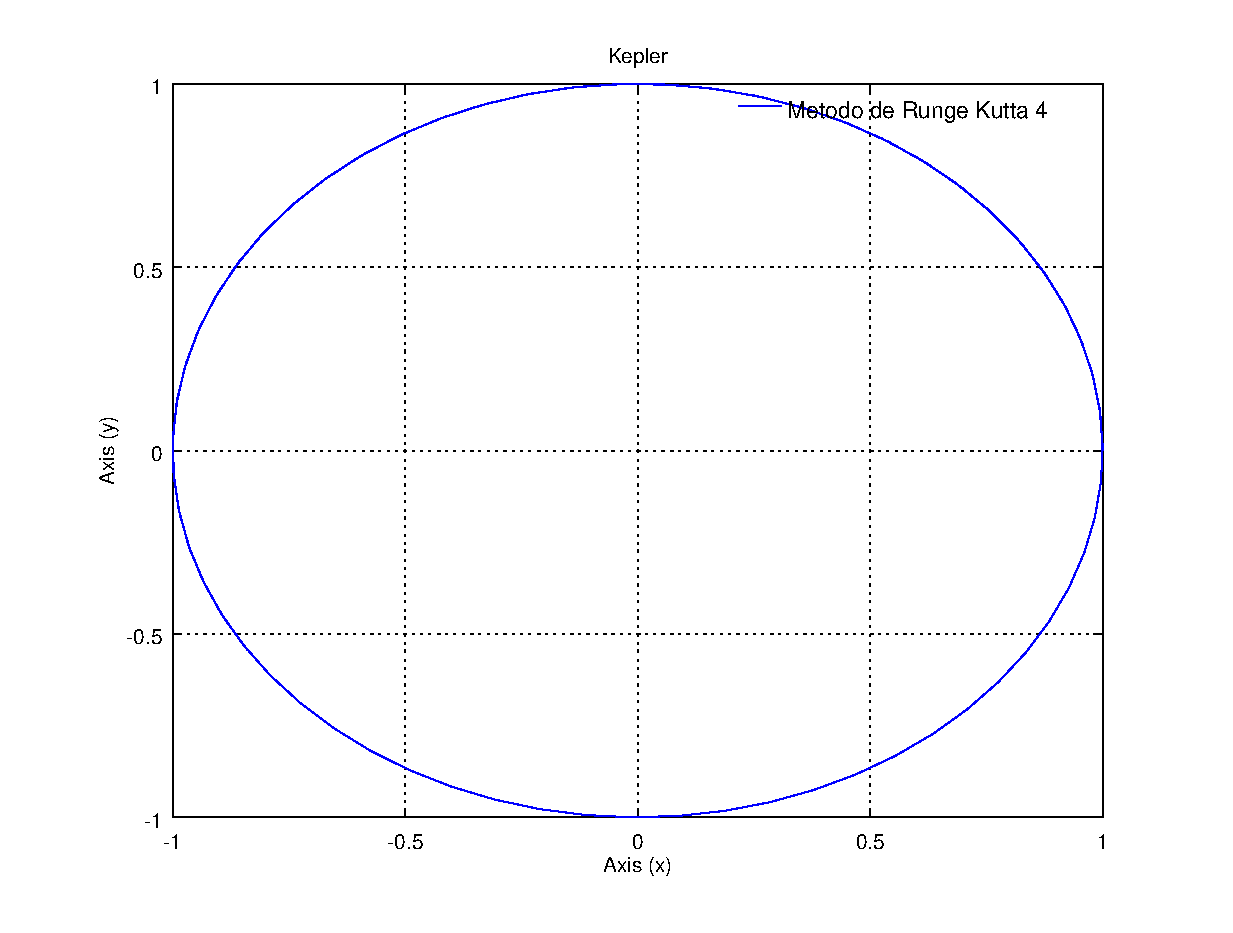
\includegraphics{k2.eps}
	}
\end{figure}
O m\'etodo de Kepler com $n = 100$ e $h = 0.1$ para o vetor inicial,
\[\left [ 
	\begin{array}{c}
		0 \\
		1 \\
		0 \\
		1
	\end{array}
\right ] 
\]
\begin{figure}[!h]
	\centering
	\resizebox{0.5\width}{!}{
	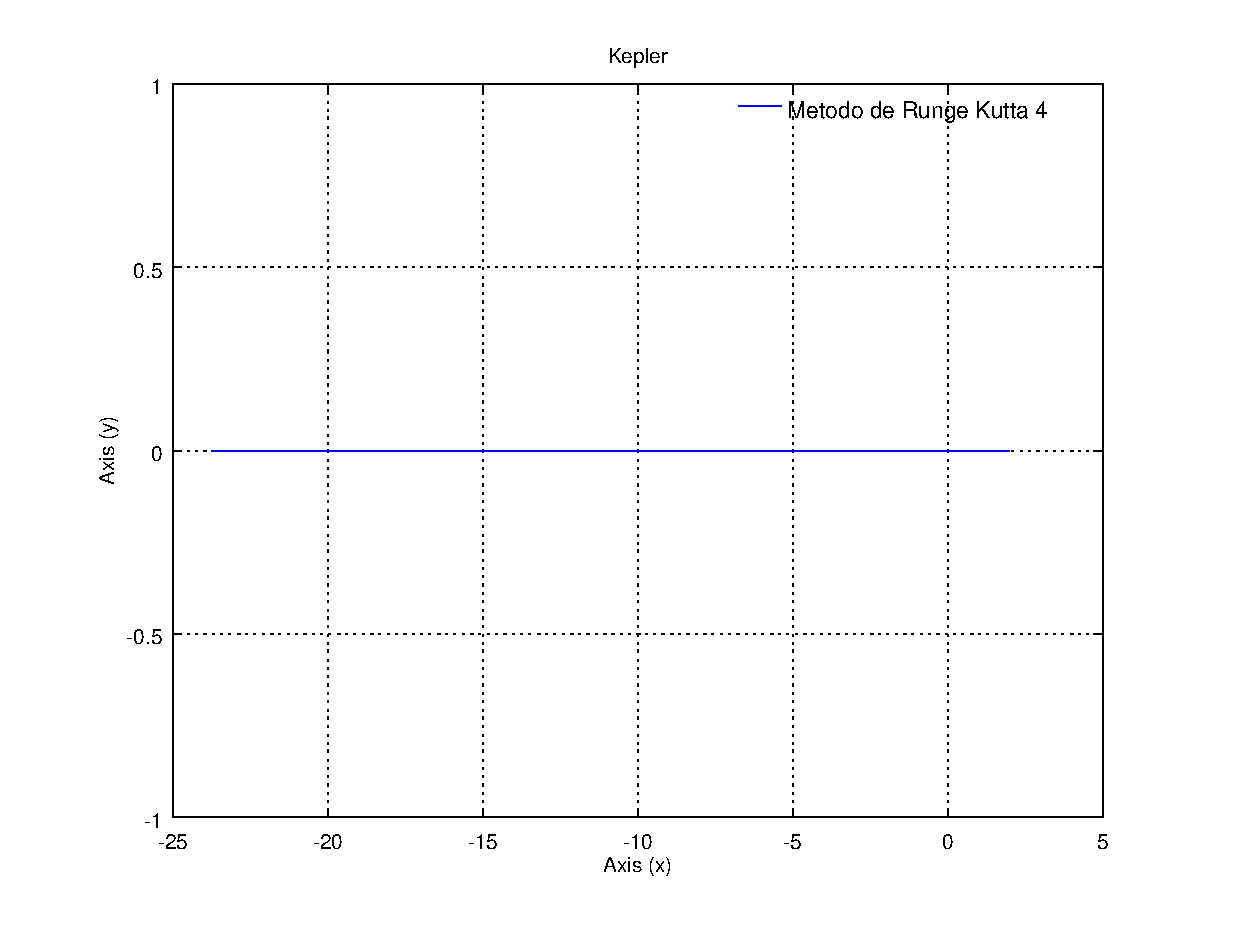
\includegraphics{k3.eps}
	}
\end{figure}
\newpage
O m\'etodo de Kepler com $n = 100$ e $h = 0.1$ para o vetor inicial,
\[\left [ 
	\begin{array}{c}
		0 \\
		1 \\
		0 \\
		0
	\end{array}
\right ] 
\]
\begin{figure}[!h]
	\centering
	\resizebox{0.5\width}{!}{
	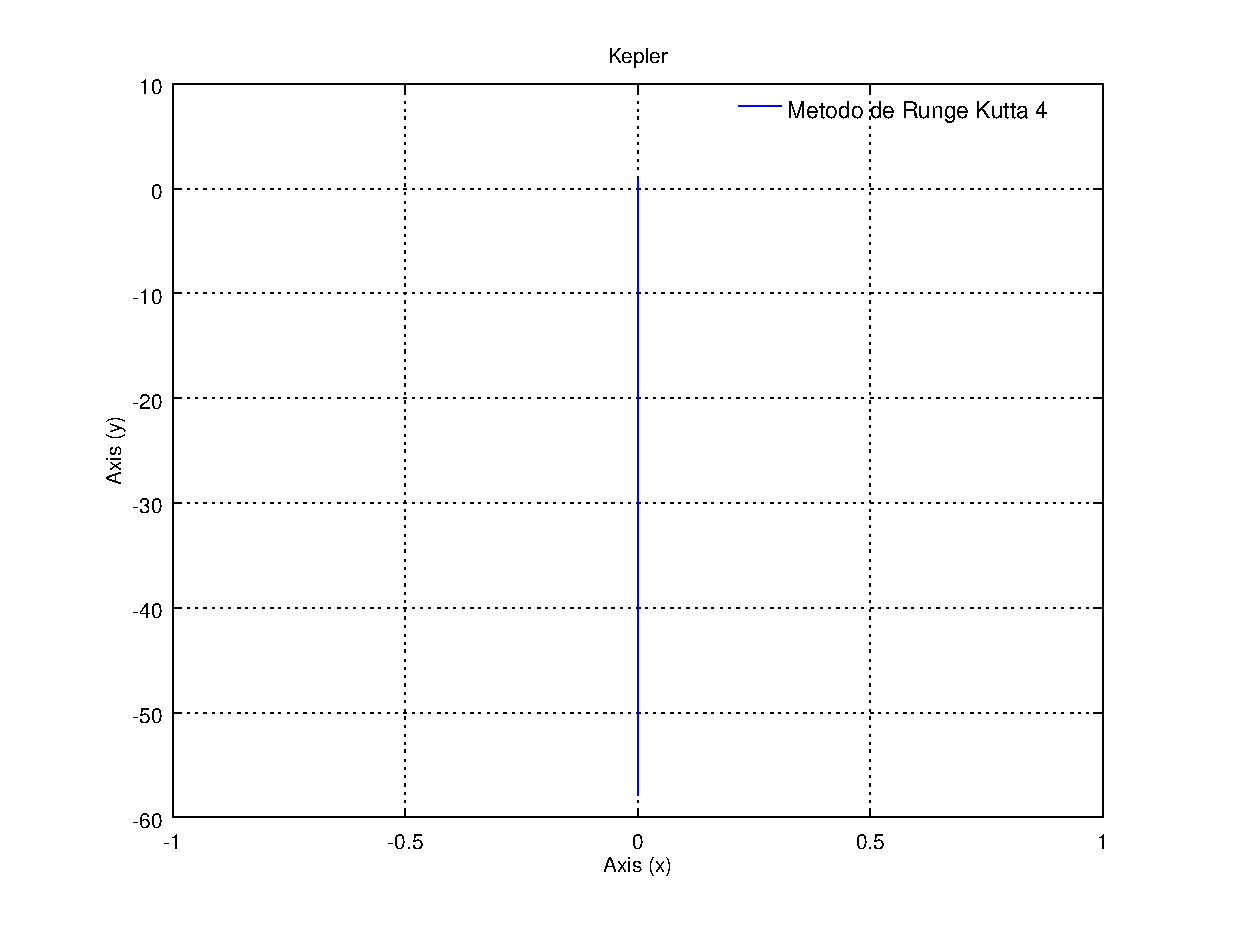
\includegraphics{k4.eps}
	}
\end{figure}


\end{document}
	
